\section{Validation}
\noindent
{\color{LightRubineRed} \rule{\linewidth}{1mm} }
%%%%%%%%%%%%%%
\subsection{Model Selection Problem} % (fold)
\label{sub:model_selection_problem}
\begin{align*}
E_{out} \approx E_{in} \approx 0
\end{align*}
selecting by $E_{in}$ is dangerous,因为模型在训练集训练过了,会overfitting \par
Model selection by Best $E_{test}$,但是测试集一般是看不到的,因此可以split出验证集。\par
% subsection model_selection_problem (end)

\subsection{Validation Set} % (fold)
\label{sub:validation_set}
$E_{val}$用于选择模型,桥接$E_{in}$和$E_{out}$.如果能保证$D_{val}$,$D_{train}$以及$D_{test}$都是iid的来自于同一个分布$P$的话,效果是有保证的。 \par
\begin{center}
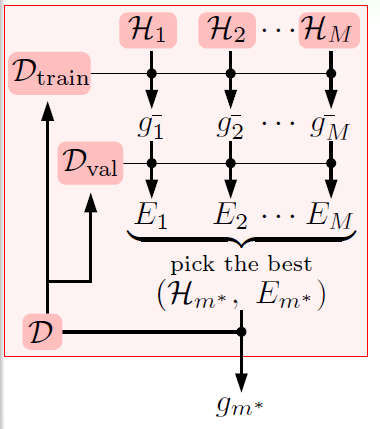
\includegraphics[width=4.5cm, height=6cm]{lecture15_1}
\end{center}
% subsection validation_set (end)

\subsection{Leave-One-Out Cross Validation} % (fold)
\label{sub:leave_one_out_cross_validation}

% subsection leave_one_out_cross_validation (end)
\subsection{V-fold Cross validation} % (fold)
\label{sub:v_fold_cross_validation}
交叉验证。
% subsection v_fold_cross_validation (end)
%%%%%%%%%%%%%%
\begin{center}
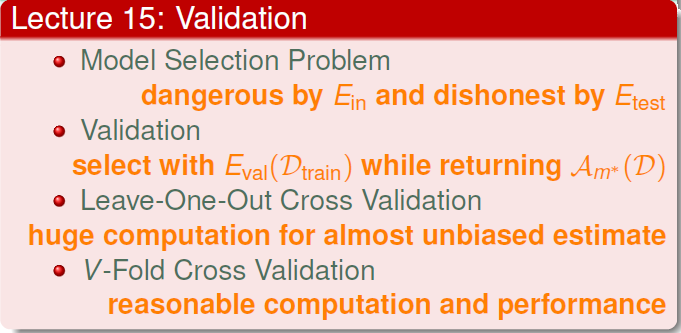
\includegraphics[width=10cm, height=5cm]{lecture15_sum}
\end{center}
\noindent
{\color{RubineRed} \rule{\linewidth}{1mm} }